%% tl-netz-totalausfall.tex
\chapter{Totalausfall des Netzes}
\label{cha:netz-totalausfall}

\begin{abstractsec}
  Habe ich an einem Rechner überhaupt keine Netzverbindung, oder kann ich ein
  ganzes Netzsegment nicht erreichen, spreche ich von einem Totalausfall.
\end{abstractsec}

\section{Ein Rechner hat überhaupt keine Netzverbindung}
\label{sec:gar-kein-netz}

\begin{abstractsec}
  Dieser Abschnitt beschäftigt sich mit dem Totalausfall des Netzwerks an
  einem Rechner.
\end{abstractsec}
\begin{normaltext}
  Manchmal kommt es vor, dass ein Rechner überhaupt keine Netzwerkverbindung
  hat. Dann bleibt nichts übrig, als dem Problem methodisch auf den Grund zu
  gehen. Dazu verwende ich den folgenden Entscheidungsbaum, um das Problem in
  Teilprobleme zu zerlegen:

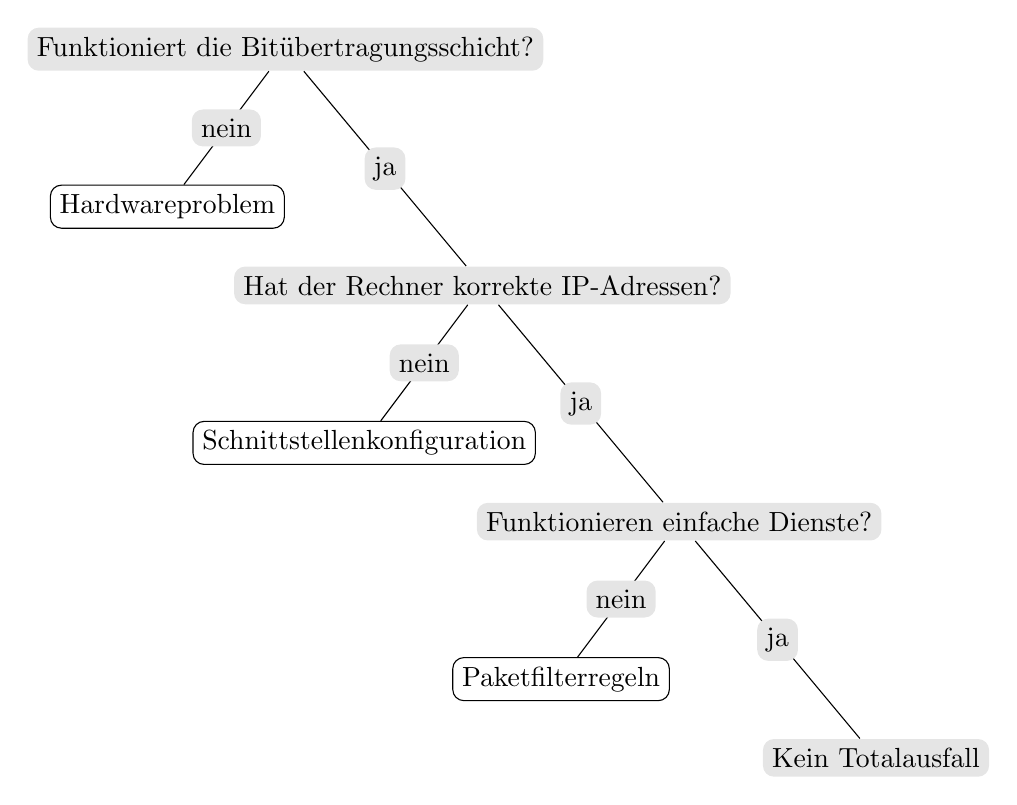
\begin{tikzpicture}
[every node/.style={fill=black!10,rounded corners,align=center},
grow=south, level distance=2cm,
level 1/.style={sibling distance=3cm},
level 2/.style={sibling distance=3cm},
]

\node{Funktioniert die Bitübertragungsschicht?}
  child{node[draw,fill=white]{Hardwareproblem}
  edge from parent node[fill=black!10]{nein}}
  child{node at +(1,-1) {Hat der Rechner korrekte IP-Adressen?}
    child{node[draw,fill=white]{Schnittstellenkonfiguration}
    edge from parent node{nein}}
    child{node at +(1,-1) {Funktionieren einfache Dienste?}
      child{node[draw,fill=white]{Paketfilterregeln}
      edge from parent node{nein}}
      child{node at +(1,-1) {Kein Totalausfall}
      edge from parent node{ja}}
    edge from parent node{ja}}
  edge from parent node{ja}};
\end{tikzpicture}

  Die allererste Frage geht dabei nach der physischen Netzverbindung, im
  OSI-Modell auch Bitübertragungsschicht genannt. Bei Hardware-Rechnern mit
  einigermaßen neuer Netzwerkkarte helfen mir die mii-tools beziehungsweise
  eth-tools, die Auskunft über die Verbindungsparameter zum Switch geben
  können. Habe ich es mit einer virtuellen Maschine zu tun, dann muss ich am
  Hostsystem die Netzwerkeinstellungen für diese VM kontrollieren.

  Auch das Programm ifconfig zeigt an, ob das betreffende Interface eine
  physikalische Verbindung hat (\verb?RUNNING?). Noch deutlicher zeigt  es
  \verb?ip link show? beziehungsweise \verb?ip addr show? (\verb?LOWER_UP?
  oder \verb?NO-CARRIER?).

  Habe ich diese Programme nicht zur Verfügung, kann ich mich vielleicht mit
  \verb?netstat -i? behelfen. Dieser Befehl zeigt eine Statistik der
  gesendeten und empfangenen Pakete an. Da in jedem Netzwerk ein gewisser
  Anteil an Broadcastpaketen unterwegs ist, sollte sich die Anzahl der
  empfangenen Datenpakete erhöhen, wenn ich den Befehl im Abstand von einigen
  Sekunden aufrufe. Um sicher zu gehen, kann ich auf einem anderen Rechner im
  gleichen Netzsegment zum Beispiel mit ping Broadcastpakete erzeugen.

  Wenn tcpdump installiert ist, kann ich auch mit
  \verb?tcpdump -n -i <schnittstelle>? auf Traffic warten. Wenn ich damit
  Traffic sehe, beende ich das Programm nicht gleich, sondern warte, bis ich
  an Hand der Datenpakete entscheiden kann, ob die Schnittstelle im richtigen
  Segment angeschlossen ist.

  Kann ich keinen Traffic nachweisen, muss ich mir die Verkabelung ansehen,
  probeweise die Kabel tauschen, den Rechner an einen anderen Switch
  anschließen und/oder in ein anderes Netzsegment. Bei virtuellen Maschinen
  schaue ich auf dem Host nach, ob andere VM ähnliche Probleme haben, ob
  vielleicht ein falscher Netzwerkanschluß zugewiesen wurde oder kontrolliere
  die entsprechenden virtuellen Interfaces auf dem Host.

  Ein kurzer Test mit \verb?iptables -L? und \verb?ebtables -L? sagt mir, ob
  vielleicht Paketfilterregeln die Verbindung unterdrücken.

  Erst wenn die Bitübertragungsschicht funktioniert, hat es überhaupt Sinn,
  sich dem nächsten Problem, der IP-Konfiguration zuzuwenden. Diese muss zum
  angeschlossenen Netzsegment passen. Eventuell ist es besser, für die Dauer
  der Fehlersuche, alle Regeln zu entfernen und die Policies auf \verb?ACCEPT?
  zu stellen.

  Habe ich vorher die Funktionalität der Schnittstelle mit tcpdump
  kontrolliert, dann habe ich eventuell schon genügend Pakete gesehen, die mir
  zeigen, ob die Schnittstelle im richtigen Segment angeschlossen ist.
  Ansonsten kann ich das jetzt nachholen.

  Habe ich tcpdump nicht an Board, weiß aber, dass DHCP im Netzwerk zur
  Verfügung steht, kann ich versuchen darüber eine IP-Adresse zu bekommen.
  Dazu stelle ich temporär die Schnittstellenkonfiguration um. Falls ich es
  noch nicht getan habe, deaktiviere ich jetzt alle Paketfilter.

\begin{Exkursbox}{Konfiguration der Netzwerkschnittstelle}
  Bei Debian: /etc/network/interfaces

  Bei Redhat: /etc/sysconfig/network-scripts/*
\end{Exkursbox}

  Kann ich DHCP nicht nutzen, so könnte ich noch versuchen mit Zero
  Configuration Networking zu anderen Rechnern in meinem Segment zu bekommen.
  Das hängt davon ab, wie das betreffende Netzwerk administriert ist.

  Habe ich nicht die Möglichkeit für Tests mit DHCP/Zero Configuration
  Networking, kann ich versuchen mit Ping bekannte und aktive Stationen in
  meinem Netzsegment zu erreichen. Antworten die Stationen nicht, aber ihre
  IP-Adressen tauchen korrekt im ARP-Cache auf (Test mit \verb?arp -an?), dann
  liegt das Problem eher an zu restriktiven Paketfiltereinstellungen der
  anderen Rechner und ich würde diese dort testweise lockern beziehungsweise
  auf den anderen Rechnern mit tcpdump oder Wireshark nachschauen, ob ich
  Datenpakete des problematischen Rechners sehen kann. Bei VMs kann ich mit
  tcpdump am zugehörigen virtuellen Interface des Hosts nachschauen.

\begin{Exkursbox}{Sperren von ICMP durch Paketfilter}
  Verweis auf übermäßiges Beschränken von ICMP-Verkehr und die Auswirkungen
  auf den Netzverkehr.
\end{Exkursbox}

Habe ich mich davon überzeugt, dass der Rechner im richtigen Netzsegment
angeschlossen ist und Stationen in diesem erreichen kann, muss ich mich nur
noch vergewissern, dass er Rechner in anderen Netzen erreichen kann.

Bei der Überprüfung der Schnittstellenkonfiguration, habe ich mich gleich mit
vergewissert, dass der Rechner das richtige Gateway kennt. Ich überzeuge mich
davon, dass die konfigurierte Konfiguration auch aktiv ist. Insbesondere
überprüfe ich:

\begin{itemize}
  \item Stimmen IP-Adresse und Netzmaske? (\verb?ip addr show?)
  \item Stimmen Gateway und Routen? (\verb?ip route show?)
  \item Kann ich das Gateway erreichen? (\verb?ping $gateway?)
\end{itemize}

\begin{Exkursbox}{IPv4-Netzmasken}
  An dieser Stelle will ich ein paar Worte zu IPv4-Netzmasken verlieren. Zu
  einer Zeit, in der IPv6 langsam an Fahrt gewinnt, mutet das vielleicht etwas
  anachronistisch an. Leider werden diese noch fast überall eingesetzt und
  sind insbesondere bei der Fehlersuche in IPv4-Netzen Grundvoraussetzung. Es
  lohnt sich daher für den Netzwerk Troubleshooter nach wie vor, diese zu
  memorieren, falls er nicht in der Lage ist, sie in annehmbarer Zeit im Kopf
  herzuleiten.

  Prinzipiell gibt es zwei Schreibweisen:
  \begin{itemize}
    \item in Bitnotation: /0 .. /32
    \item in Vierer-Notation: 0.0.0.0 .. 255.255.255.255
  \end{itemize}
  Beide Schreibweisen lassen sich in einander umrechnen. Beide müssen
  beherrscht werden, da einige Programme nur die eine oder die andere
  verwenden können.

  Bei der Umrechnung helfen uns die ehemaligen Netzwerkklassen mit ihrer
  Größenunterteilung in 8-Bit-Grenzen.
  In der folgenden Tabelle habe ich die drei Klassen A, B, C um die Notation
  für das gesamte IPv4-Netz auf der einen Seite und für einen einzelnen Host
  auf der anderen Seite ergänzt:

  \begin{tabular}{l|c|l|r}
    & Bit & Vierergruppen & Anzahl Hosts \\
    \hline
    gesamtes Netz & /0 & 0.0.0.0 & > 4 Milliarden \\
    Class A Size & /8 & 255.0.0.0 & > 16 Millionen \\
    Class B Size & /16 & 255.255.0.0 & > 65 Tausend \\
    Class C Size & /24 & 255.255.255.0 & 254 \\
    Host & /32 & 255.255.255.255 & 1 \\
  \end{tabular}

  Interessanter sind die Subnetz- oder CIDR-Masken. Für diese gehe ich von der
  Netzmaske der nächstgrößeren Klasse aus und füge die entsprechende Anzahl
  Bits (1..7) hinzu. In Viererschreibweise ändert sich die Position, die bei
  der klassenbasierten Adresse die erste 0 hat.

  \begin{tabular}{c|c|c|l}
    Bits & VS & Binär & Netzadressen \\
    \hline
    /+1 & 128 & 80 & 0, 128 \\
    /+2 & 192 & C0 & 0, 64, 128, 192 \\
    /+3 & 224 & E0 & 0, 32, 64, 96, 128, \ldots \\
    /+4 & 240 & F0 & 0, 16, 32, 48, 64, \ldots \\
    /+5 & 248 & F8 & 0, 8, 16, 24, 32, \ldots \\
    /+6 & 252 & FC & 0, 4, 8, 12, 16, \ldots \\
    /+7 & 254 & FE & 0, 2, 4, 6, 8, \ldots \\
  \end{tabular}

  Die Netzadresse gibt an, an welcher Adresse das betreffende Netz beginnt.
  Diese Adresse kann nicht für Hosts vergeben werden. In der Tabelle habe ich
  nur maximal die ersten vier aufgeführt. Die weiteren ergeben sich, indem man
  die erste oder zweite zu allen Netzadressen der nächsthöheren Zeile addiert.
  Die zugehörige Broadcast-Adresse ist die Adresse des nächsten Netzwerkes mit
  gleicher Bitmaske, vermindert um 1.

  Nehmen wir als Beispiel einen Host mit der IPv4-Adresse
  \verb?10.21.32.43/29?. Die Netzmaske ist \verb?/24+5?, in Vierernotation
  \verb?255.255.255.248?. Die Netzadresse ist \verb?10.21.32.40?, die
  Broadcastadresse ist \verb?10.21.32.47?.
\end{Exkursbox}

Anschließend versuche ich mit ping einen Rechner in einem anderen
Netzsegment zu erreichen, der zum Beispiel von anderen Stationen
aus diesem Segment erreicht werden kann. Kann ich trotz korrekter
IP-Konfiguration und deaktiviertem Paketfilter auf dem Problemrechner keine
Rechner in anderen Segmenten erreichen, muss ich auf dem Gateway nachsehen, ob
die Datenpakete des Problemrechners dort vorbeikommen. Sehe ich diese am
Gateway, kann ich den Problemrechner bei der Fehlersuche hinter mir lassen,
vielleicht noch einen Dauerping einschalten und muss mich bei der Problemsuche
dem Netz zuwenden.

\end{normaltext}

%\subsection{Seiteneffekte}
%\label{sec:seiteneffekte}

%\subsection{Einschränkung der Umsetzung}
%\label{sec:einschr-der-umsetz}

%\begin{notes}
%\item Was nicht geht
%\item geht auch nicht
%\item und auch das
%\end{notes}

\section{Ein oder mehrere Netzsegmente sind nicht erreichbar}
\label{sec:ausfall-netzsegment}

\begin{normaltext}
  Beim Ausfall eines oder mehrerer Netzsegmente unterscheide ich zunächst, ob
  ich mich in einem der betroffenden Segmente befinde, oder nicht.

  Bin ich direkt in dem betroffenen Netzsegment - zum Beispiel, wenn der
  Ausfall mir von außerhalb gemeldet wird - untersuche ich zunächst, ob ich
  innerhalb des Netzsegmentes, vor allem zum Gateway Verbindung habe.
  Dabei kann ich gegebenenfalls auf das Vorgehen aus
  \ref{sec:gar-kein-netz} zurückgreifen.
  Anschließend versuche ich Kontakt zu dem Netzsegment zu bekommen, aus dem
  die Meldung kam. Bekomme ich keinen Kontakt, vermute ich ein Routingproblem.

  Bin ich außerhalb der betroffenen Netzsegmente, schaue ich als erstes, ob
  die Routen dorthin in Ordnung sind. Dabei kann mir das Programm traceroute
  helfen. Genauere Auskunft bekomme ich auf den Gateways oder anderen
  Rechnern, die an den Routingprotokollen teilnehmen. Fehlen die Routen, oder
  weisen sie in die falsche Richtung, muss ich das Routingproblem untersuchen.
  Sind die Routen in Ordnung, aber ich bekomme keine Verbindung, versuche ich
  vom Gateway des betreffenden Netzsegmentes eine Verbindung zu den Rechnern
  zu bekommen. Ist das möglich, dann handelt es sich möglicherweise um ein
  Konfigurationsproblem der betreffenden Rechner - dieses kann auch durch
  fehlerhafte Angaben vom DHCP-Server kommen.
\end{normaltext}

\begin{notes}
\item Entscheidungsbaum!
\end{notes}

\subsection*{Routingprobleme}
\label{sec:routingprobleme}

\begin{notes}
\item Routingprotokolle
\item OSPF: BDR hatte falschen Neighbor (openbsd, GeNUScreen)
\item Routersoftware quagga
\end{notes}

\subsection*{Rückroute fehlt}
\label{sec:rueckroute-fehlt}

\begin{notes}
\item Problem: Routen scheinen zu stimmen, keine Antwortpakete
\item Analyse: traceroute, analyse des letzten Hops und desjenigen danach
\item Ursache: Rückroute fehlt
\end{notes}

%%% Local Variables: 
%%% mode: latex
%%% TeX-master: "arbeit-hauptdatei"
%%% End: 
%%% vim: set sw=2 ts=2 tw=78 et si:
